%% Chapter 8 : Generation Forecasting using 

\section{Introduction to Artificial Neural Networks}
\
\
\
\
Artificial Neural Networks (ANN) are a type of machine learning model, they are inspired from the biological neural networks present in the brains of the animals. Being highly non-linear, data driven and with a self adaptive approach; ANN's are a powerful tool for modelling phenomenons whose underlying principles and/or data relationships are unknown. They try to imitate the learning process of the human brain, and when trained properly can correlate patterns between input data and the corresponding target data; moreover they can predict outcomes for new independent data. Their adaptive nature replaces traditional programming with learning in problem solving. This helps in developing computational models for applications where there is little or incomplete understanding of the problem to be solved but where training data is readily available.\\

\textbf{Characterisctics of ANN's:}

\begin{itemize}

\item ANNs possess mapping capability, hence they can map input data to the corresponding output data.

\item ANNs possess learning capability, hence they can be trained with available data of a problem and be tested for inference on unknown data. They can identify new outcomes for data sets on which they were previously never trained.

\item ANNs possess generalizing capability, hence they can predict new outcomes from past trends.

\item ANNs are robust and fault tolerant, hence they can capture capture complete patterns from partial and/or noisy patterns.

\item ANNs can process information in parallel, at high speed and in a distributed manner.

\end{itemize}

\newpage

\section{Artificial Neuron}
\
\
\
\
The artificial neuron is the building block of the ANN. The Fig (\ref{figc8h1}) shows the diagrammatic representation of an artificial neuron.

\begin{figure}[H]
\centering
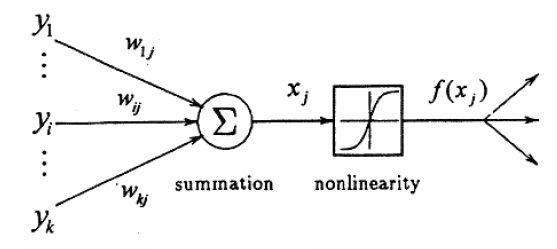
\includegraphics[scale=1]{ANNImg1}
\caption{Artificial Neuron Model}
\label{figc8h1} %% to refer use, \ref{}
\end{figure}

It consists of the weights one each for the connecting input signals, a summation unit which sums the product of the weight and the incoming input for all inputs and a activation function (which is usually a non-linear function). It also sometimes consist of a bias. The mathematical model of the artificial neuron is described by the following equations:

\begin{equation}
\label{ANN1}

\textit{f}(x_{j})=f \left (\alpha_{j} + \sum\limits_{i=1}^{k}w_{ij}y_{i}  \right )
  
\end{equation}\\
where,\\
$ \textit{f} $ = It is the activation function of the artificial neuron \\
$ \alpha_{j} $ = It is the bias associated with the $j^{th}$ neuron in the network \\
$ k $ = It is total number of inputs connected to the $j^{th}$ neuron in the network 
$ w_{ij} $ = It is weight associated with the connection between the $i^{th}$ input and the $j^{th}$ neuron \\
$ y_{i} $ = It is the $i^{th}$ input connected to the neuron \\
$ \textit{f}(x_{j}) $ = It is the out put of the $j^{th}$ neuron


The Fig (\ref{ANNActFunc}) shows the different activation functions which can be used in the design of the artificial neurons.

\begin{figure}[H]    
\begin{center}
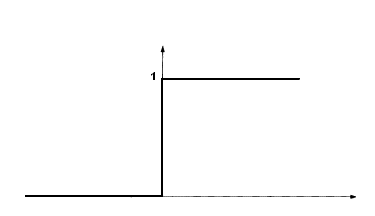
\includegraphics[width=.4\textwidth]{ANNImg4}
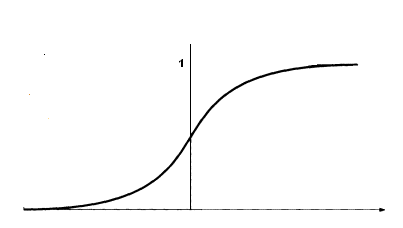
\includegraphics[width=.4\textwidth]{ANNImg5}
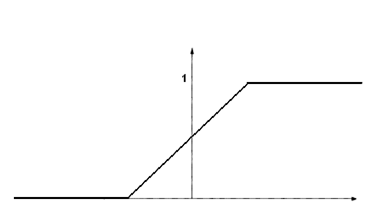
\includegraphics[width=.4\textwidth]{ANNImg6}
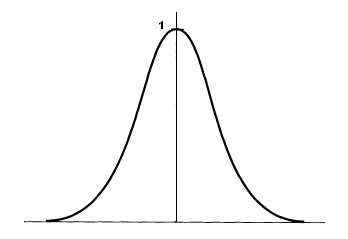
\includegraphics[width=.4\textwidth]{ANNImg7}
\end{center}
\caption{Different Activation Functions: Upper Left - Unit Step, Upper Right - Sigmoid, LowerLeft - Piecewise Linear and LowerRight - Gaussian}    
\label{ANNActFunc}
\end{figure} 

These artificial neurons form the unit processing element s of an artificial neural network. The arrangement (network architectures) of these artificial neurons and its subsequent training leads to development of ANN models which solve real world problems whose principles and data relationships are little or incompletely understood.

\section{ANN Architectures}
\
\
\
\
Neural network architectures are the structures developed by the interconnection of artificial neurons. The two most widely used ANN architectures are: Feed Forward Network and Recurrent Network.

\textbf{Feed Forward Network:}\\

In these networks information flows in one direction i.e from the input layer passing through the hidden layers and finally to the output layer. There are no feedbacks i.e. the output of any layer does not affect the same or the preceding layer. The Fig (\ref{figc8h2}) illustrates a feed forward neural network.

\begin{figure}[H]
\centering
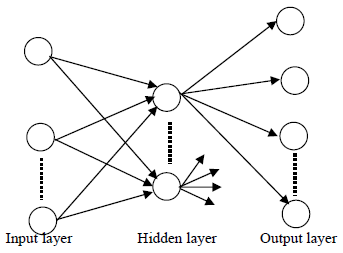
\includegraphics[scale=1]{ANNImg2}
\caption{Schematic of Feed-Forward Network}
\label{figc8h2} %% to refer use, \ref{}
\end{figure}

\textbf{Recurrent Network:}\\

These artificial neural networks consist of feedbacks (atleast one). The possible feedbacks are: feedback between two layers or feedback to a single neuron (self-feedback links). The Fig (\ref{figc8h3}) shows a recurrent neural network where the feedback is provided from the output layer to input layer.

\begin{figure}[H]
\centering
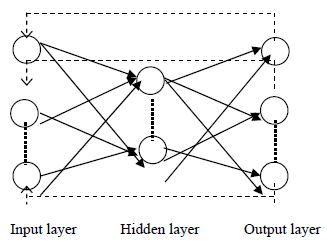
\includegraphics[scale=1]{ANNImg3}
\caption{Artificial Neuron Model}
\label{figc8h3} %% to refer use, \ref{}
\end{figure}

The more specific neural network architesctures used widely for real world problem solving are: Multi-Layer Perceptron Networks (MLP), Radial Bias Function Networks and Kohonen Self Organizing Feature Maps.

\textbf{Multi-Layer Perceptron Network:}\\

It is the most popular form of the ANN architecture. It has the following properties:

\begin{itemize}

\item Has any number of inputs

\item Has one or more hidden layers with any number of units

\item Uses linear combination functions in the input layers

\item Generally uses sigmoid activation functions in the hidden layers

\item Has any number of outputs with any activation function

\item Has connections between the input layer and the first hidden layer, hidden layer and hidden layer, and between hidden layer and output layer

\end{itemize}

The Fig (\ref{figc8h4}) illustrates a Multi-Layer Perceptron Network with a single hidden layer.

\begin{figure}[H]
\centering
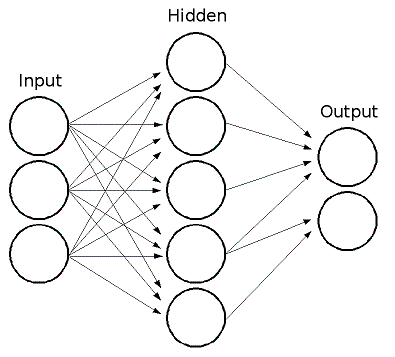
\includegraphics[scale=1]{ANN_MLP}
\caption{Multi-Layer Perceptron Architecture}
\label{figc8h4} %% to refer use, \ref{}
\end{figure}

MLP's are known as universal approximators and can  be used when we have little prior knowledge of the relationship between the inputs and the targets. Usually one hidden layer with sufficient number of neurons is enough for creating a good model, but sometimes more hidden layers with less number of neurons can improve generalization.\\

\textbf{Radial Bias Function Network:}\\

A Radial Bias Function Network (RBF) is similar to a MLP but with only one hidden layer. The properties of RBF are as follows:

\begin{itemize}

\item Has any number of inputs

\item Typically has only one hidden layer with any number of units

\item Uses radial combination functions in the hidden layers, based on the squared Euclidean distance between the input vector and the weight vector

\item Typically uses exponential or softmax activation functions in the hidden layer, in which the network is a Gaussian RBF Network

\item Has any number of outputs with any activation function

\item has connections between the input layer and the hidden layer, and between hidden layer and the output layer.

\end{itemize}

The Fig (figc8h5}) illustrates a RBF Network.

\begin{figure}[H]
\centering
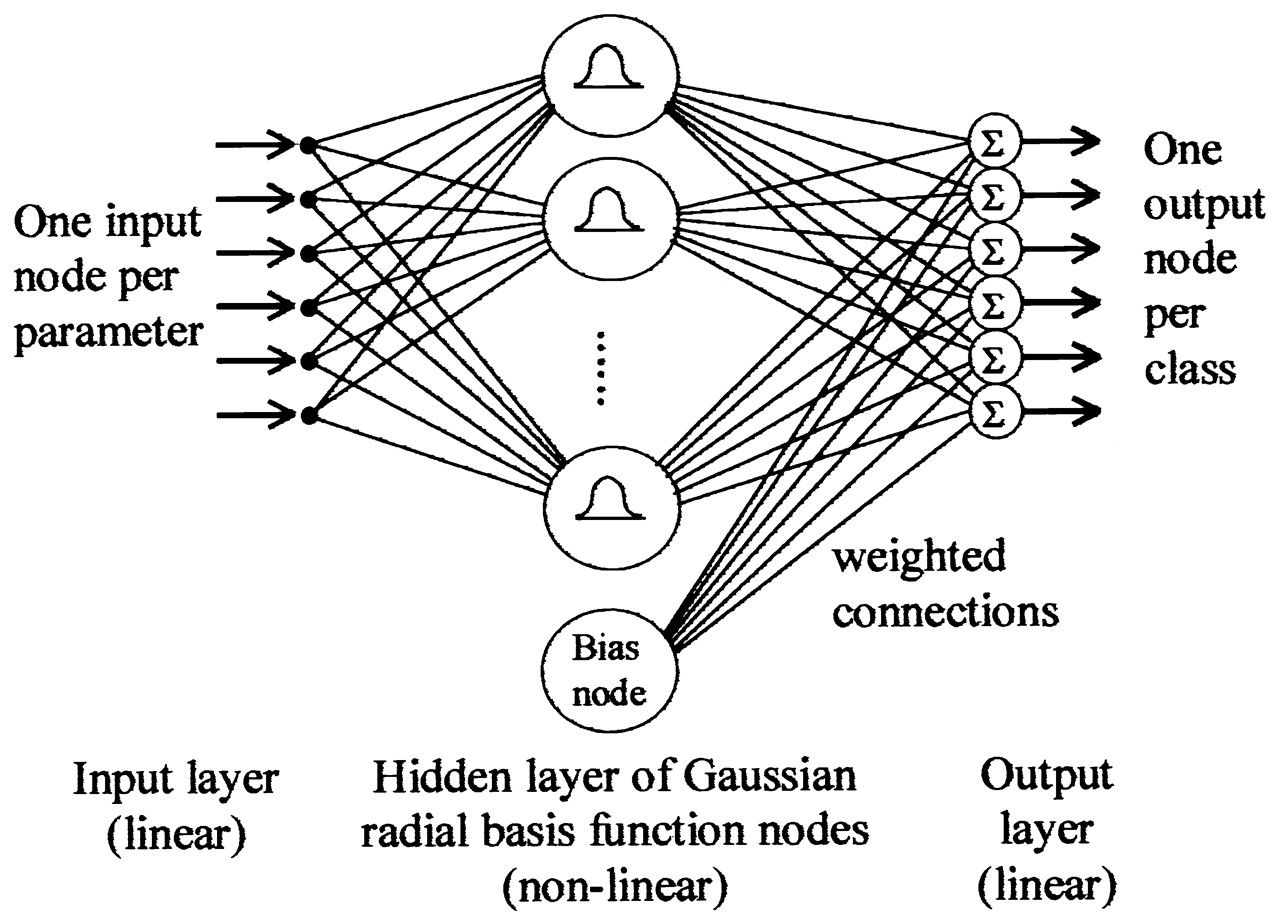
\includegraphics[scale=0.25]{ANN_RBF}
\caption{Artificial Neuron Model}
\label{figc8h5} %% to refer use, \ref{}
\end{figure}

Gaussian RBF's are said to be local-processing networks as the  effect of a hidden unit is usually concentrated in a local area centered at the weight vector ; as opposed to the MLP's which are said to be distributed-processing networks as the effect of a hidden unit cn be distributed over the entire input space.\\

\textbf{Kohonen Self Organizing Feature Maps:}\\

These are used quite diffeently from other ANN networks. Most of the ANN networks are designed for supervised learning tasks, but the self organizing Maps (SOFM) are primarily designed for unsupervised learning tasks. They help to lear the structure of data and hence oten very useful for exploratory data analysis of complex data. They care also used for novelty detection. It learns to rcognize clusters in the training data and then respond to them in a fitting manner. A SOFM consists of only two layers: an input layer, and an output layer of radial units. The Fig (\ref{figc8h6}) illustrates a Kohonen (SOFM) network.

\begin{figure}[H]
\centering
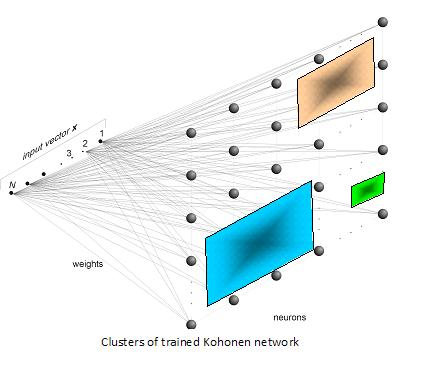
\includegraphics[scale=0.5]{ANN_Kohonen}
\caption{Artificial Neuron Model}
\label{figc8h6} %% to refer use, \ref{}
\end{figure}


\section{Training Methods}
\
\
\
\
Learning methods for neural networks can be classified into three basic types, which are given as follows:

\begin{enumerate}

\item \blindtext \textbf{Supervised Learning:} In this learning method every input pattern that is used to train the network is associated with the target or the desired pattern. A teacher is assumed to be present during the learning/training process, when a comparison is made between the network's computed output and the correct expected output, to determine the error. The error can then be used to change the network parameters (weights and biases), which result in an improvement in performance.

\item \blindtext \textbf{Unsupervised Learning:}In this learning method, the target output is not presented to the network. It is as if there is no teacher to present the desired patterns. However, the network leans of its own by discovering and adapting to the structural features in the input patterns. 

\item \blindtext \textbf{Reinforced Learning:} In this learning method, a teacher is available, but does not present the expected answer; however only indicates if the computed answer is correct or incorrect. The information provided helps the network in its learning process. A reward is given for a correct answer and a penalty for a wrong answer. But, this learning method is not very popular.

\end{enumerate

\section{ANN Applications}
\
\
\
\
The real world applications of ANN consist of a large spectrum of categories as listed below:

\begin{itemize}

\item Function approximation, or regression analysis, including time series prediction, fitness approximation and modeling

\item Classification, including pattern and sequenxce recognition, novelty detectiona nd sequential decision making

\item Data processing, including filtering, clustering, blind source separation and compression

\end{itemize}

\newpage

\section{Process Flow for Forecasting using ANN}
\
\
\
\
The Fig (\ref{figc8h7}) shows the schematic of the process flow for the development of the ANN model for forecasting.

\begin{figure}[H]
\centering
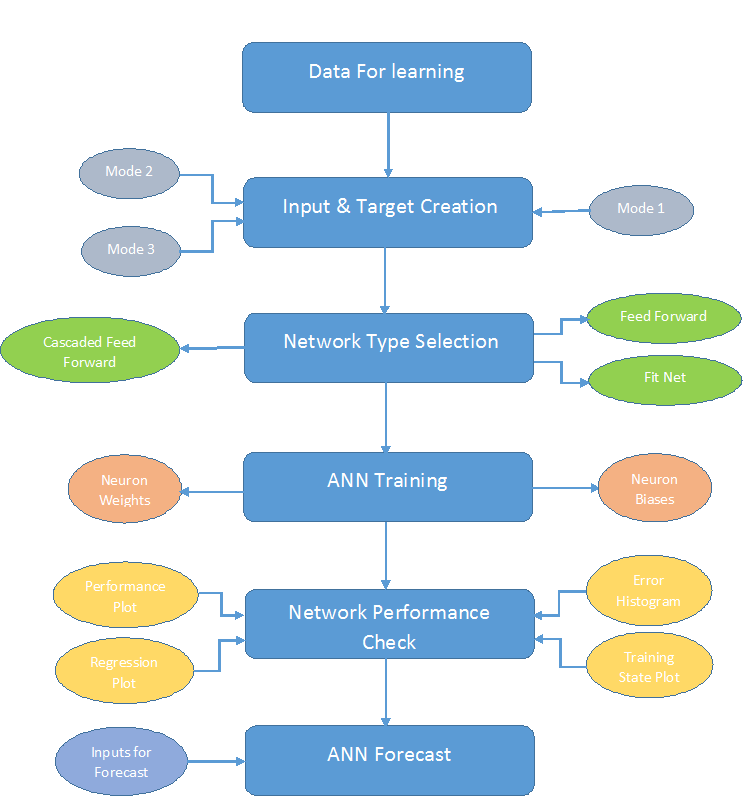
\includegraphics[scale=0.8]{ANN_Flow}
\caption{Schematic of ANN Model Development for Forecasting}
\label{figc8h7} %% to refer use, \ref{}
\end{figure}

\newpage

\section{Results}
\
\
\
\
The results for generation forecasting using ANN have been produced for the GSEC 1MW SPVP. The training data is of 11 months from November 2014 to September 2015. The ANN models trained on this data have been used to generate intra-hour weather variable forecasts for the month of October 2015. The ANN models have been developed using three different types of input data (Mode1, Mode2 and Mode3) with three different network architectures (Fitnet [FN], Feedforward Net [FF] and Cascaded Feedforward Net [CFF]) and five different hidden network configurations (5-Neurons, 10-Neurons, 15-Neurons, 10-10- Neurons and 10-10-10-neurons). All the results in the subsequent sections are for the $2^{nd}$ of October 2015 for all the modes, architectures and the hidden network configuration. The forecasted weather variables form the ANN models have been fed as inputs to the solar energy estimation app to generate the intra-hour generation forecast.


\subsection{Input Type - Mode1}
\
\
\
\
In Mode1 the Input training matrix consists of the [Day, Month, Year,Time] columns with the Target Training Matrix consisting of the corresponding [Wind Speed, Temperature, Irradiance] columns. The results are given in the following sections which are divided based on the hidden network configurations and each graph consists of the comparison of the actual variable with he forecasted variable from the three different ANN architectures. 

\subsubsection{ANN Architecture - Hidden Nodes [5]}
\
\
\
\

\begin{figure}[H]
\centering
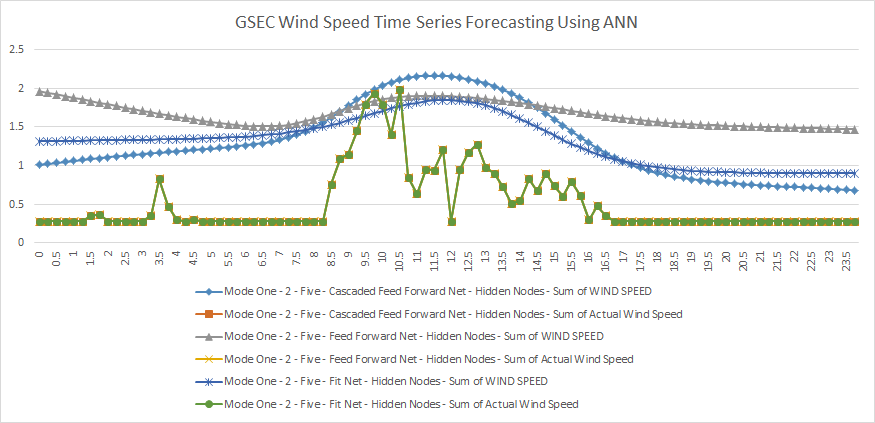
\includegraphics[scale=0.5]{ANNmOne5w}
\caption{Comparison Of Different ANN Architectures (FN,FF,CFF) For Forecasting Of Intra-Hour Wind Speed In Mode 1 With Network [5]}
\label{ANNResImg1} %% to refer use, \ref{}
\end{figure}

\begin{figure}[H]
\centering
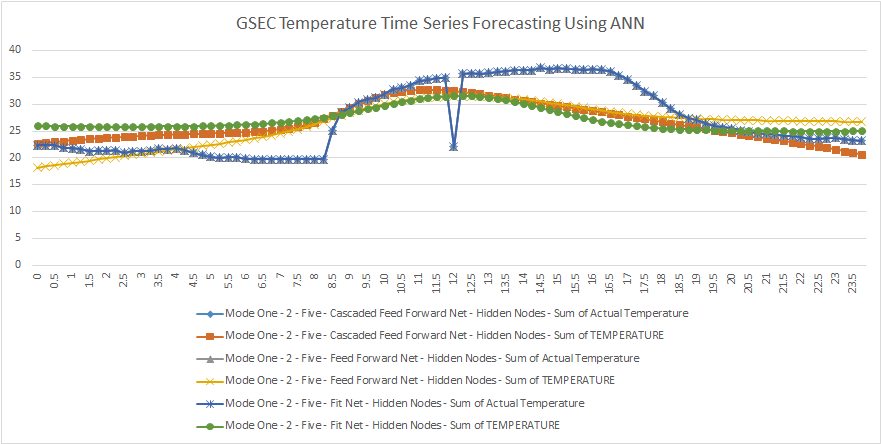
\includegraphics[scale=0.5]{ANNmOne5t}
\caption{Comparison Of Different ANN Architectures (FN,FF,CFF) For Forecasting Of Intra-Hour Temperature In Mode 1 With Network [5]}
\label{ANNResImg2} %% to refer use, \ref{}
\end{figure}

\begin{figure}[H]
\centering
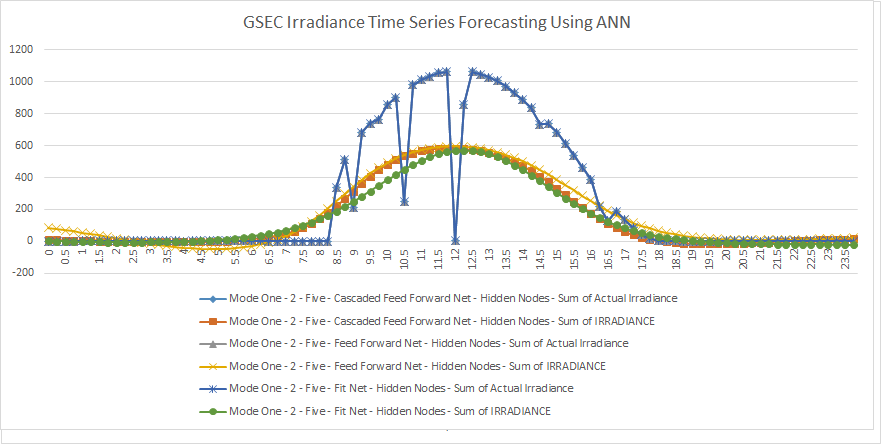
\includegraphics[scale=0.5]{ANNmOne5i}
\caption{Comparison Of Different ANN Architectures (FN,FF,CFF) For Forecasting Of Intra-Hour Irradiance In Mode 1 With Network [5]}
\label{ANNResImg3} %% to refer use, \ref{}
\end{figure}

\begin{figure}[H]
\centering
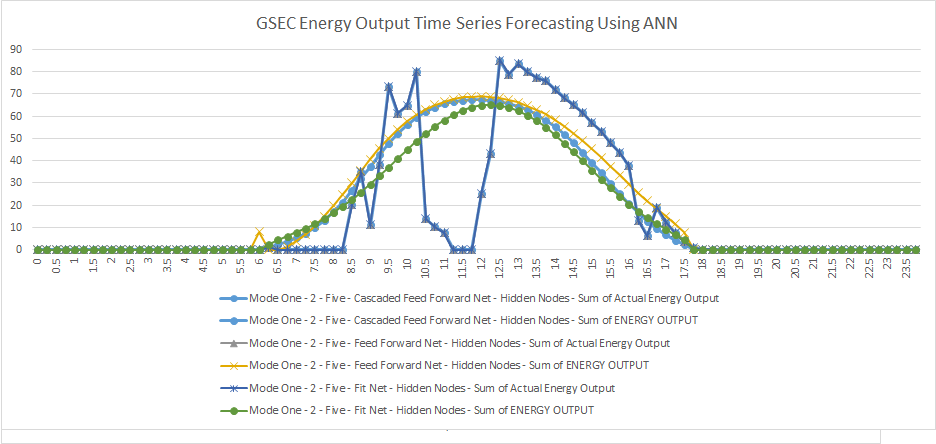
\includegraphics[scale=0.5]{ANNmOne5e}
\caption{Comparison Of Different ANN Architectures (FN,FF,CFF) For Forecasting Of Intra-Hour Energy In Mode 1 With Network [5]}
\label{ANNResImg4} %% to refer use, \ref{}
\end{figure}

\newpage

\subsubsection{ANN Architecture - Hidden Nodes [10]}
\
\
\
\

\begin{figure}[H]
\centering
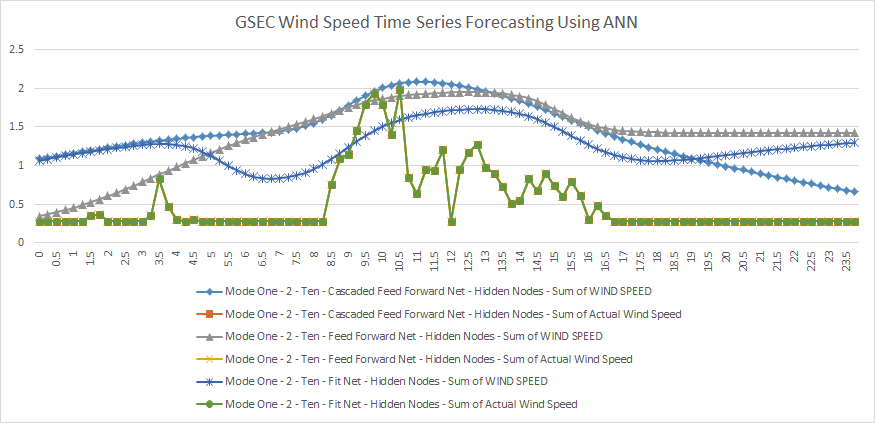
\includegraphics[scale=0.5]{ANNmOne10w}
\caption{Comparison Of Different ANN Architectures (FN,FF,CFF) For Forecasting Of Intra-Hour Wind Speed In Mode 1 With Network [10]}
\label{ANNResImg5} %% to refer use, \ref{}
\end{figure}

\begin{figure}[H]
\centering
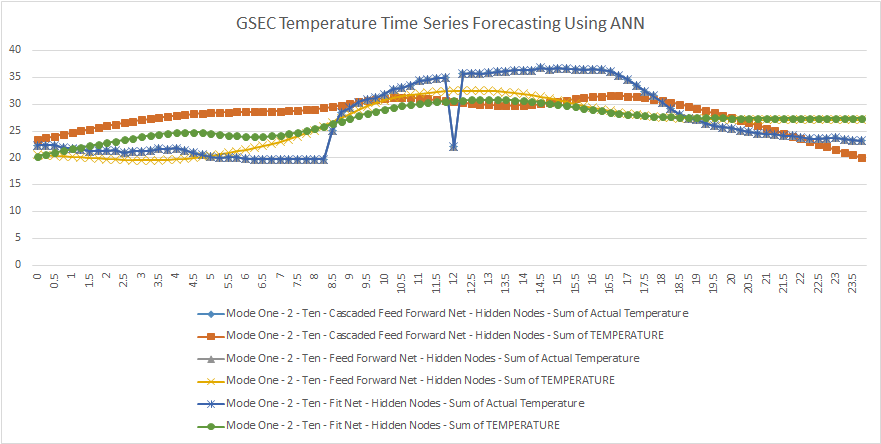
\includegraphics[scale=0.5]{ANNmOne10t}
\caption{Comparison Of Different ANN Architectures (FN,FF,CFF) For Forecasting Of Intra-Hour Temperature In Mode 1 With Network [10]}
\label{ANNResImg6} %% to refer use, \ref{}
\end{figure}

\begin{figure}[H]
\centering
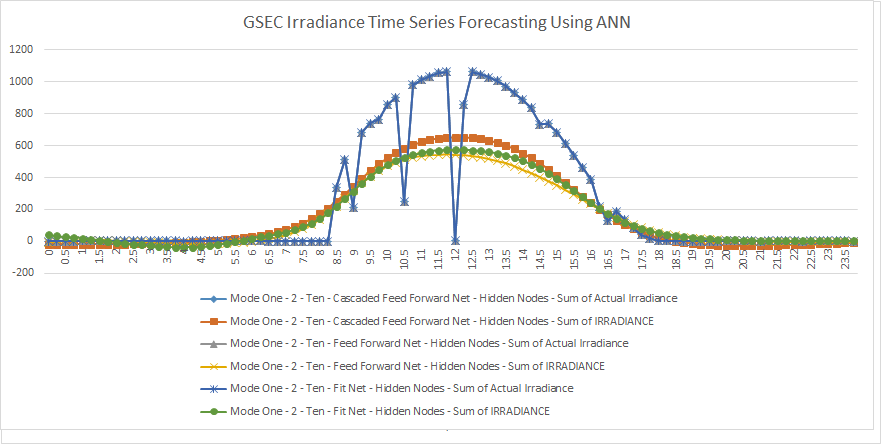
\includegraphics[scale=0.5]{ANNmOne10i}
\caption{Comparison Of Different ANN Architectures (FN,FF,CFF) For Forecasting Of Intra-Hour Irradiance In Mode 1 With Network [10]}
\label{ANNResImg7} %% to refer use, \ref{}
\end{figure}

\begin{figure}[H]
\centering
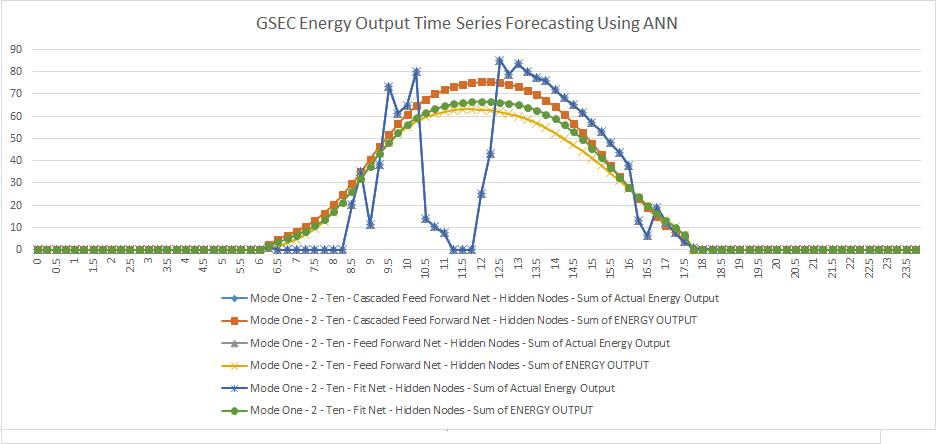
\includegraphics[scale=0.5]{ANNmOne10e}
\caption{Comparison Of Different ANN Architectures (FN,FF,CFF) For Forecasting Of Intra-Hour Energy In Mode 1 With Network [10]}
\label{ANNResImg8} %% to refer use, \ref{}
\end{figure}

\subsubsection{ANN Architecture - Hidden Nodes [15]}
\
\
\
\

\begin{figure}[H]
\centering
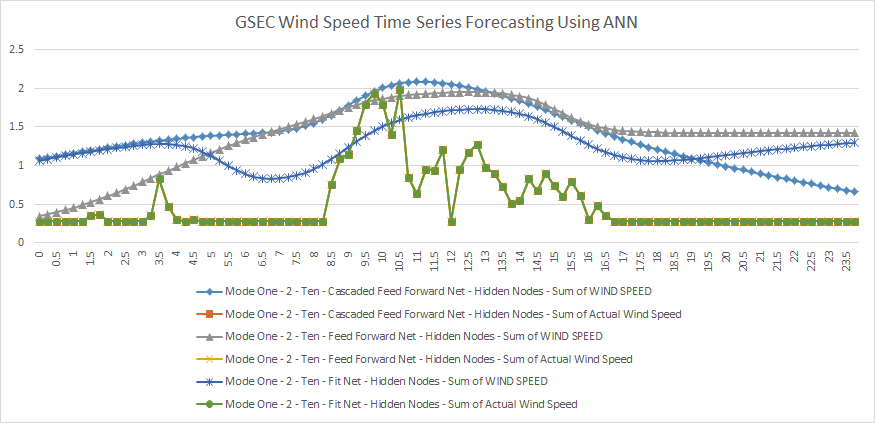
\includegraphics[scale=0.5]{ANNmOne15w}
\caption{Comparison Of Different ANN Architectures (FN,FF,CFF) For Forecasting Of Intra-Hour Wind Speed In Mode 1 With Network [15]}
\label{ANNResImg9} %% to refer use, \ref{}
\end{figure}

\begin{figure}[H]
\centering
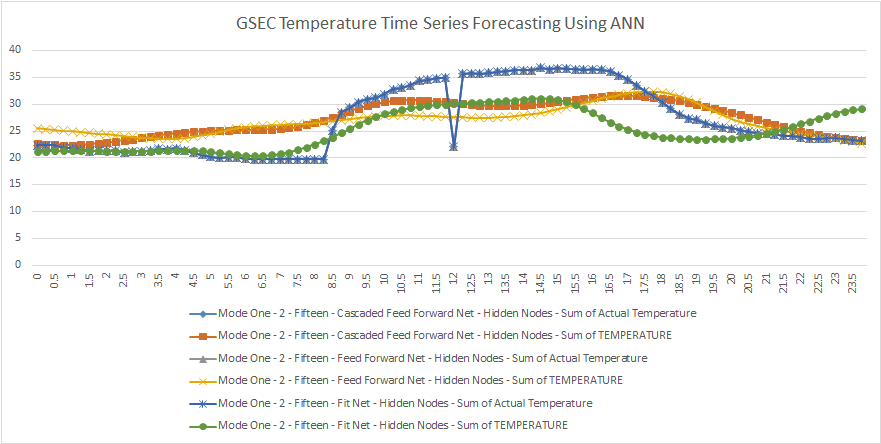
\includegraphics[scale=0.5]{ANNmOne15t}
\caption{Comparison Of Different ANN Architectures (FN,FF,CFF) For Forecasting Of Intra-Hour Temperature In Mode 1 With Network [15]}
\label{ANNResImg10} %% to refer use, \ref{}
\end{figure}

\begin{figure}[H]
\centering
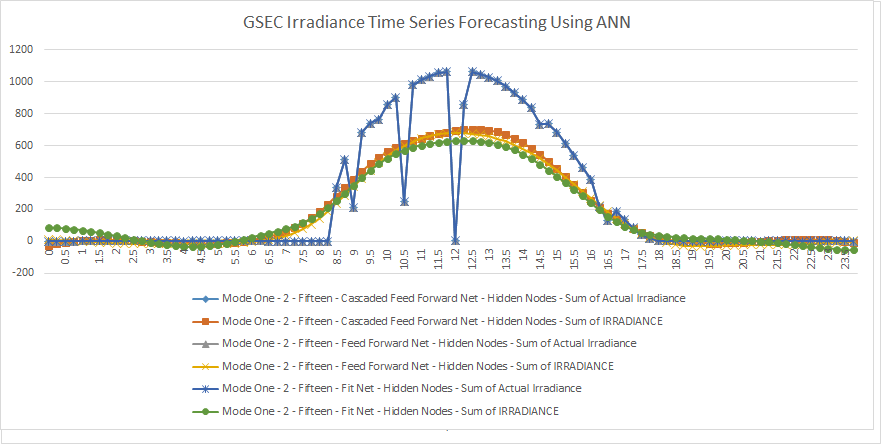
\includegraphics[scale=0.5]{ANNmOne15i}
\caption{Comparison Of Different ANN Architectures (FN,FF,CFF) For Forecasting Of Intra-Hour Irradiance In Mode 1 With Network [15]}
\label{ANNResImg11} %% to refer use, \ref{}
\end{figure}

\begin{figure}[H]
\centering
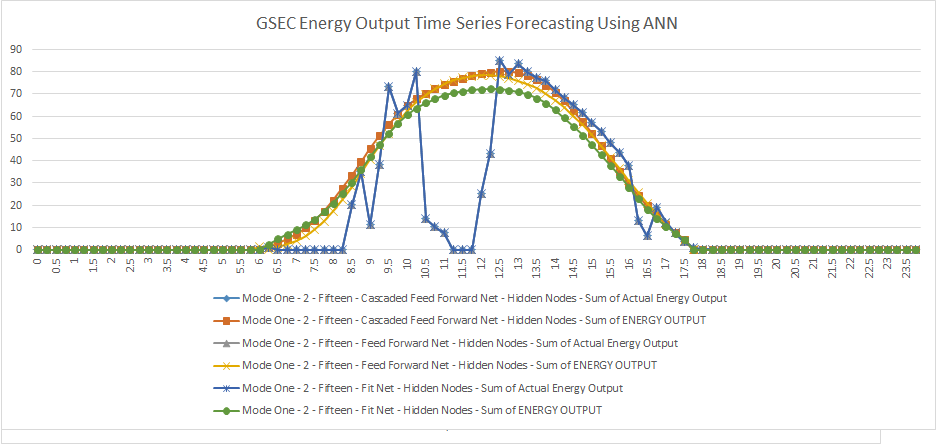
\includegraphics[scale=0.5]{ANNmOne15e}
\caption{Comparison Of Different ANN Architectures (FN,FF,CFF) For Forecasting Of Intra-Hour Energy In Mode 1 With Network [15]}
\label{ANNResImg12} %% to refer use, \ref{}
\end{figure}


\subsubsection{ANN Architecture - Hidden Nodes [10-10]}
\
\
\
\

\begin{figure}[H]
\centering
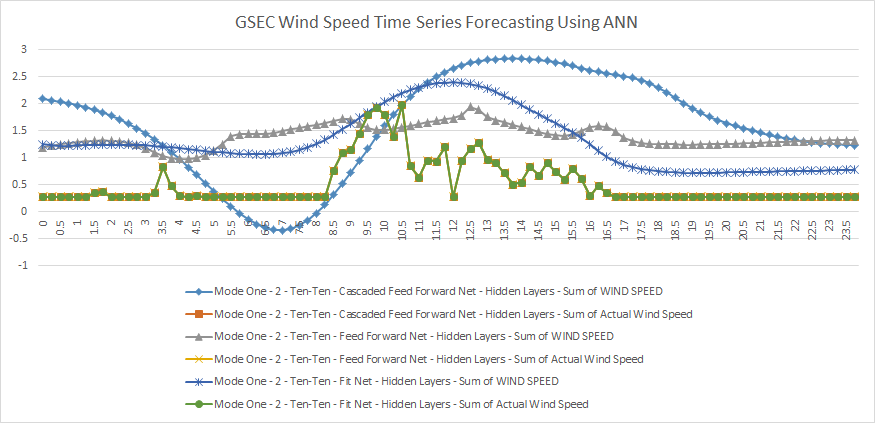
\includegraphics[scale=0.5]{ANNmOne10-10w}
\caption{Comparison Of Different ANN Architectures (FN,FF,CFF) For Forecasting Of Intra-Hour Wind Speed In Mode 1 With Network [10-10]}
\label{ANNResImg13} %% to refer use, \ref{}
\end{figure}

\begin{figure}[H]
\centering
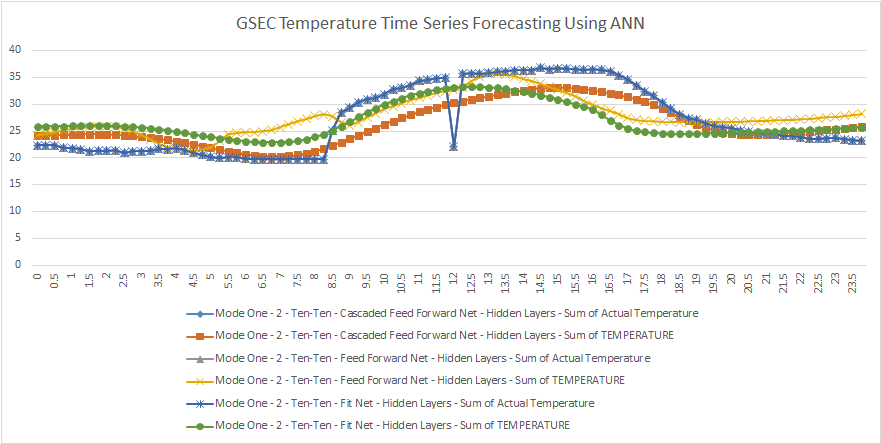
\includegraphics[scale=0.5]{ANNmOne10-10t}
\caption{Comparison Of Different ANN Architectures (FN,FF,CFF) For Forecasting Of Intra-Hour Temperature In Mode 1 With Network [10-10]}
\label{ANNResImg14} %% to refer use, \ref{}
\end{figure}

\begin{figure}[H]
\centering
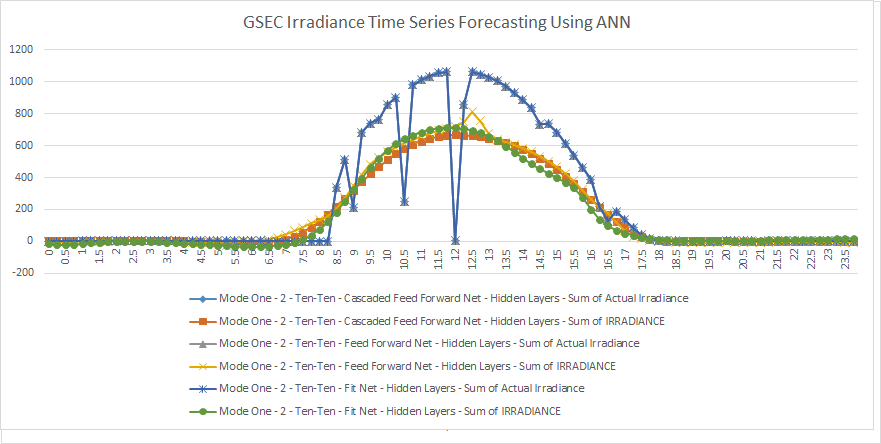
\includegraphics[scale=0.5]{ANNmOne10-10i}
\caption{Comparison Of Different ANN Architectures (FN,FF,CFF) For Forecasting Of Intra-Hour Irradiance In Mode 1 With Network [10-10]}
\label{ANNResImg15} %% to refer use, \ref{}
\end{figure}

\begin{figure}[H]
\centering
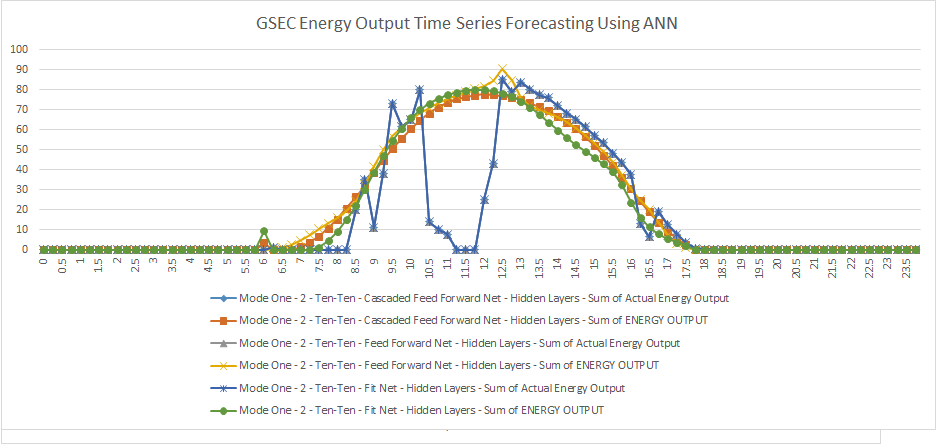
\includegraphics[scale=0.5]{ANNmOne10-10e}
\caption{Comparison Of Different ANN Architectures (FN,FF,CFF) For Forecasting Of Intra-Hour Energy In Mode 1 With Network [10-10]}
\label{ANNResImg16} %% to refer use, \ref{}
\end{figure}

\subsubsection{ANN Architecture - Hidden Nodes [10-10-10]}
\
\
\
\

\begin{figure}[H]
\centering
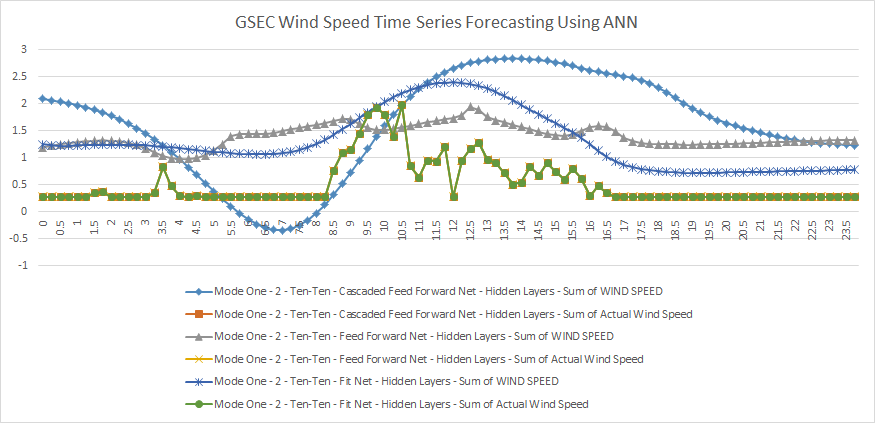
\includegraphics[scale=0.5]{ANNmOne10-10-10w}
\caption{Comparison Of Different ANN Architectures (FN,FF,CFF) For Forecasting Of Intra-Hour Wind Speed In Mode 1 With Network [10-10-10]}
\label{ANNResImg17} %% to refer use, \ref{}
\end{figure}

\begin{figure}[H]
\centering
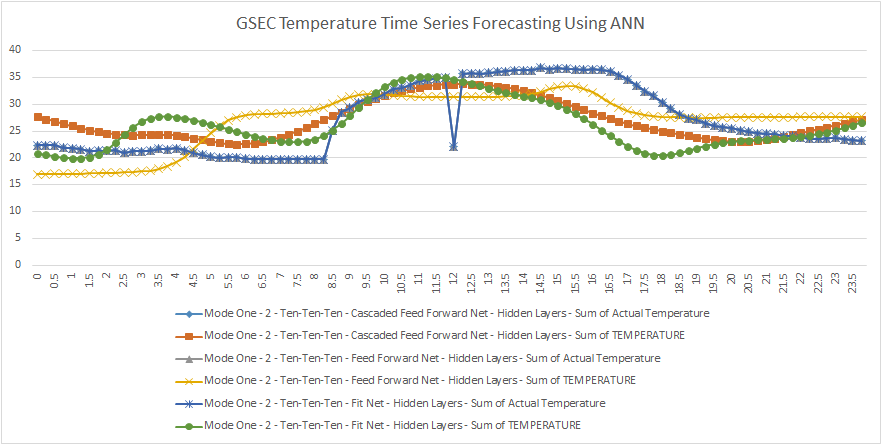
\includegraphics[scale=0.5]{ANNmOne10-10-10t}
\caption{Comparison Of Different ANN Architectures (FN,FF,CFF) For Forecasting Of Intra-Hour Temperature In Mode 1 With Network [10-10-10]}
\label{ANNResImg18} %% to refer use, \ref{}
\end{figure}

\begin{figure}[H]
\centering
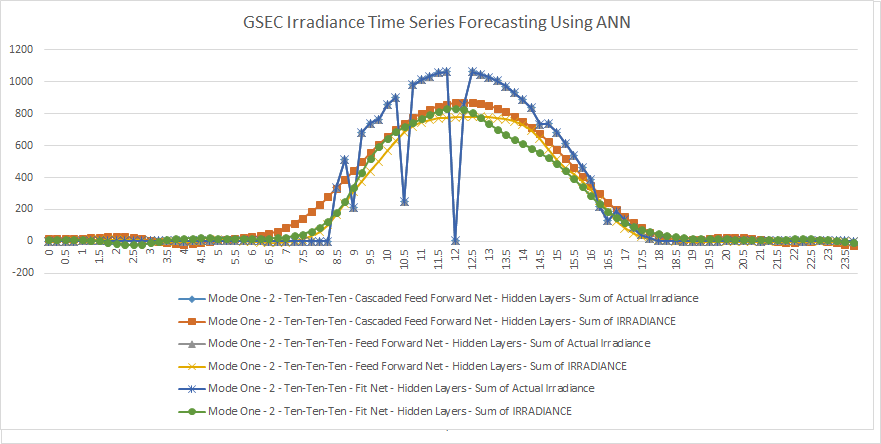
\includegraphics[scale=0.5]{ANNmOne10-10-10i}
\caption{Comparison Of Different ANN Architectures (FN,FF,CFF) For Forecasting Of Intra-Hour Irradiance In Mode 1 With Network [10-10-10]}
\label{ANNResImg19} %% to refer use, \ref{}
\end{figure}

\begin{figure}[H]
\centering
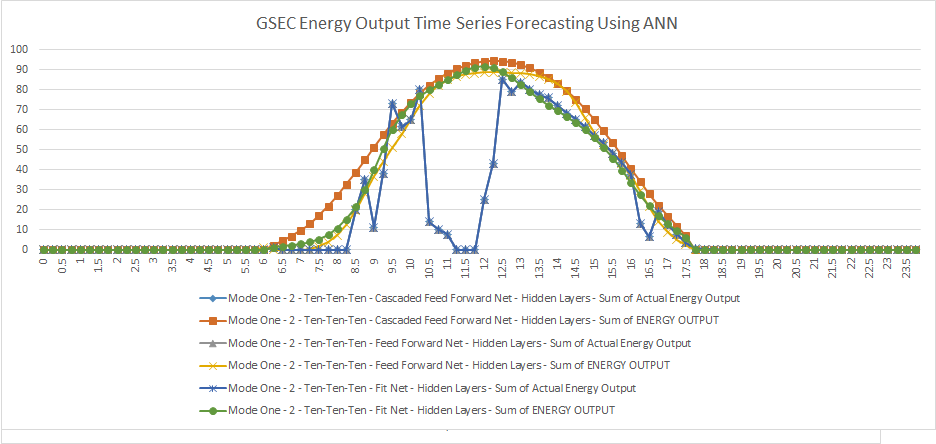
\includegraphics[scale=0.5]{ANNmOne10-10-10e}
\caption{Comparison Of Different ANN Architectures (FN,FF,CFF) For Forecasting Of Intra-Hour Energy In Mode 1 With Network [10-10-10]}
\label{ANNResImg20} %% to refer use, \ref{}
\end{figure}


\subsection{Input Type - Mode2}
\
\
\
\
In Mode2 the Input training matrix consists of the [Day, Month, Year,Time] columns with the Target Training Matrix consisting of the corresponding [Wind Speed, Temperature, Irradiance, Previous Wind Speed, Previous Temperature, Previous Irradiance] columns. The results are given in the following sections which are divided based on the hidden network configurations and each graph consists of the comparison of the actual variable with he forecasted variable from the three different ANN architectures. 

\subsubsection{ANN Architecture - Hidden Nodes [5]}
\
\
\
\

\begin{figure}[H]
\centering
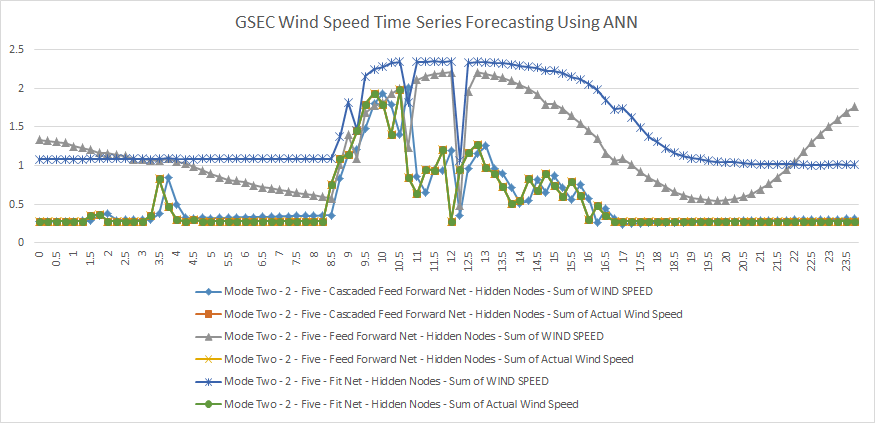
\includegraphics[scale=0.5]{ANNmTwo5w}
\caption{Comparison Of Different ANN Architectures (FN,FF,CFF) For Forecasting Of Intra-Hour Wind Speed In Mode 2 With Network [5]}
\label{ANNResImg21} %% to refer use, \ref{}
\end{figure}

\begin{figure}[H]
\centering
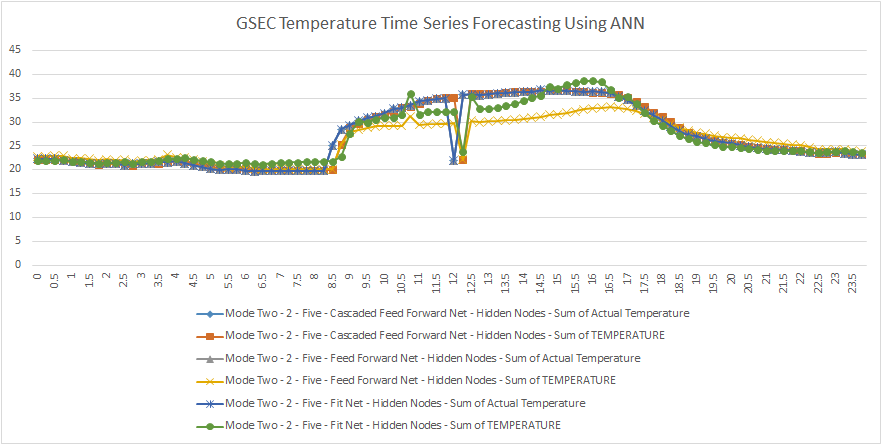
\includegraphics[scale=0.5]{ANNmTwo5t}
\caption{Comparison Of Different ANN Architectures (FN,FF,CFF) For Forecasting Of Intra-Hour Temperature In Mode 2 With Network [5]}
\label{ANNResImg22} %% to refer use, \ref{}
\end{figure}

\begin{figure}[H]
\centering
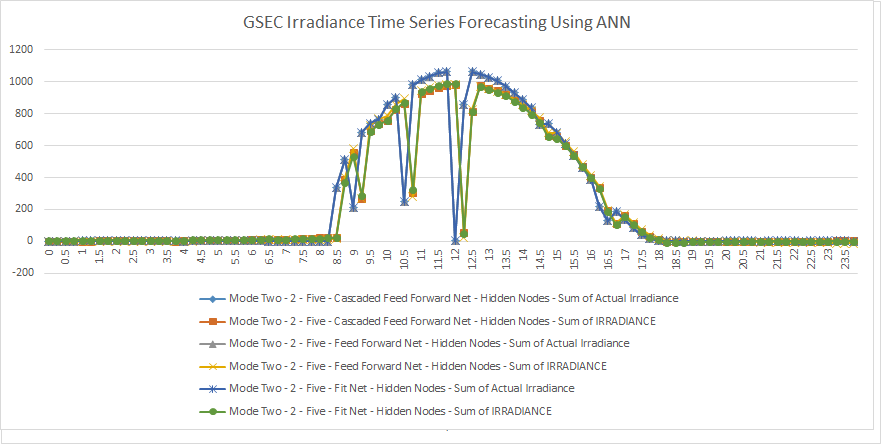
\includegraphics[scale=0.5]{ANNmTwo5i}
\caption{Comparison Of Different ANN Architectures (FN,FF,CFF) For Forecasting Of Intra-Hour Irradiance In Mode 2 With Network [5]}
\label{ANNResImg23} %% to refer use, \ref{}
\end{figure}

\begin{figure}[H]
\centering
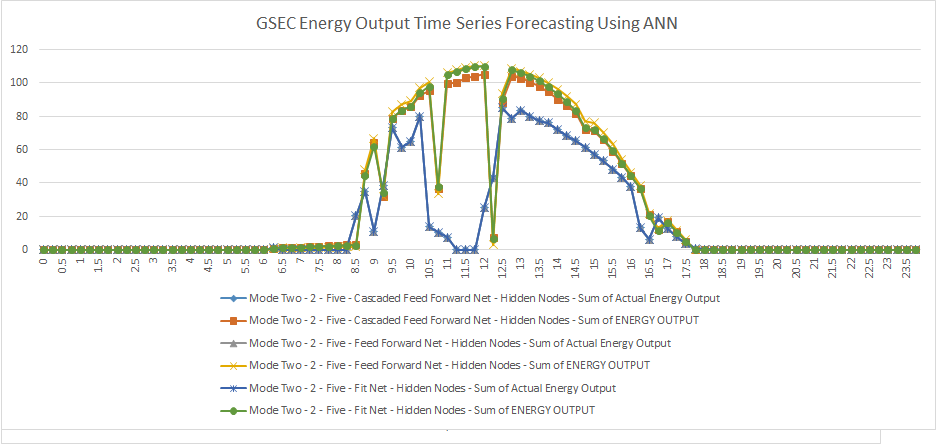
\includegraphics[scale=0.5]{ANNmTwo5e}
\caption{Comparison Of Different ANN Architectures (FN,FF,CFF) For Forecasting Of Intra-Hour Energy In Mode 2 With Network [5]}
\label{ANNResImg24} %% to refer use, \ref{}
\end{figure}

\newpage

\subsubsection{ANN Architecture - Hidden Nodes [10]}
\
\
\
\

\begin{figure}[H]
\centering
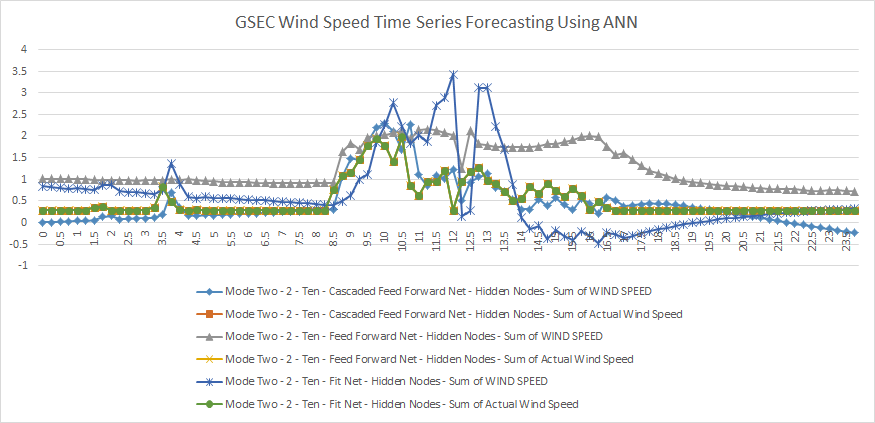
\includegraphics[scale=0.5]{ANNmTwo10w}
\caption{Comparison Of Different ANN Architectures (FN,FF,CFF) For Forecasting Of Intra-Hour Wind Speed In Mode 2 With Network [10]}
\label{ANNResImg25} %% to refer use, \ref{}
\end{figure}

\begin{figure}[H]
\centering
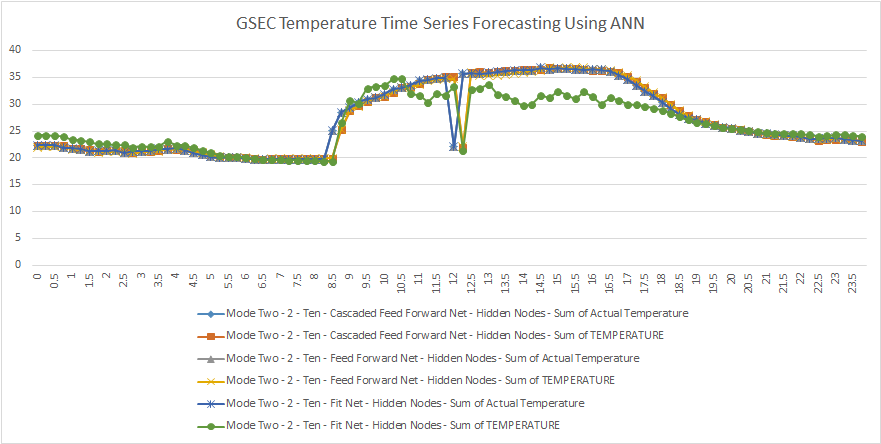
\includegraphics[scale=0.5]{ANNmTwo10t}
\caption{Comparison Of Different ANN Architectures (FN,FF,CFF) For Forecasting Of Intra-Hour Temperature In Mode 2 With Network [10]}
\label{ANNResImg26} %% to refer use, \ref{}
\end{figure}

\begin{figure}[H]
\centering
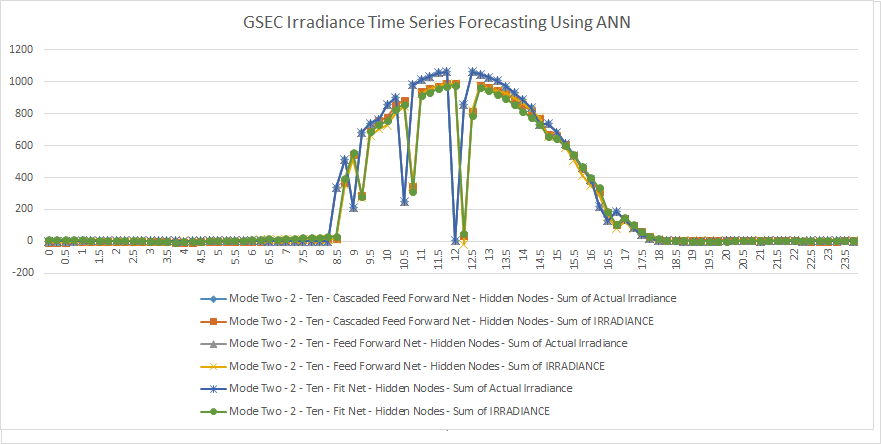
\includegraphics[scale=0.5]{ANNmTwo10i}
\caption{Comparison Of Different ANN Architectures (FN,FF,CFF) For Forecasting Of Intra-Hour Irradiance In Mode 2 With Network [10]}
\label{ANNResImg27} %% to refer use, \ref{}
\end{figure}

\begin{figure}[H]
\centering
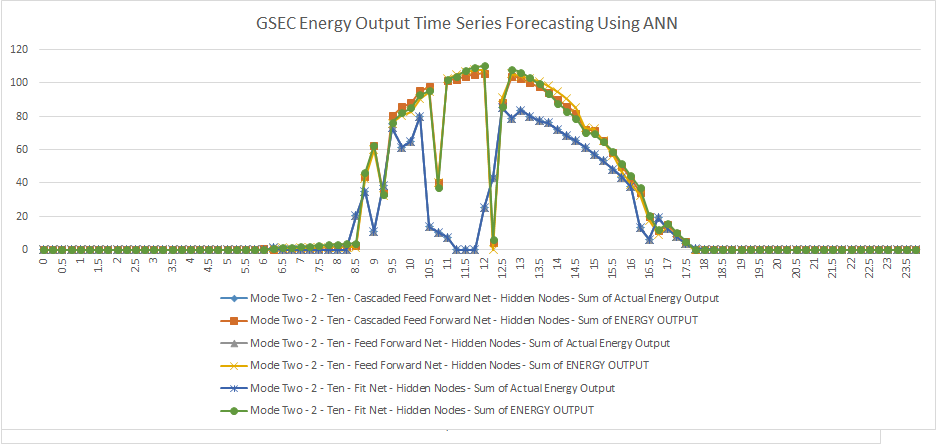
\includegraphics[scale=0.5]{ANNmTwo10e}
\caption{Comparison Of Different ANN Architectures (FN,FF,CFF) For Forecasting Of Intra-Hour Energy In Mode 2 With Network [10]}
\label{ANNResImg28} %% to refer use, \ref{}
\end{figure}

\subsubsection{ANN Architecture - Hidden Nodes [15]}
\
\
\
\

\begin{figure}[H]
\centering
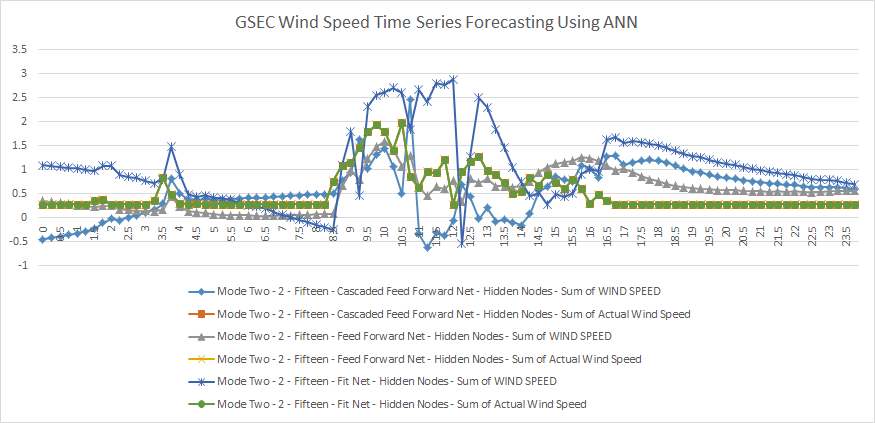
\includegraphics[scale=0.5]{ANNmTwo15w}
\caption{Comparison Of Different ANN Architectures (FN,FF,CFF) For Forecasting Of Intra-Hour Wind Speed In Mode 2 With Network [15]}
\label{ANNResImg29} %% to refer use, \ref{}
\end{figure}

\begin{figure}[H]
\centering
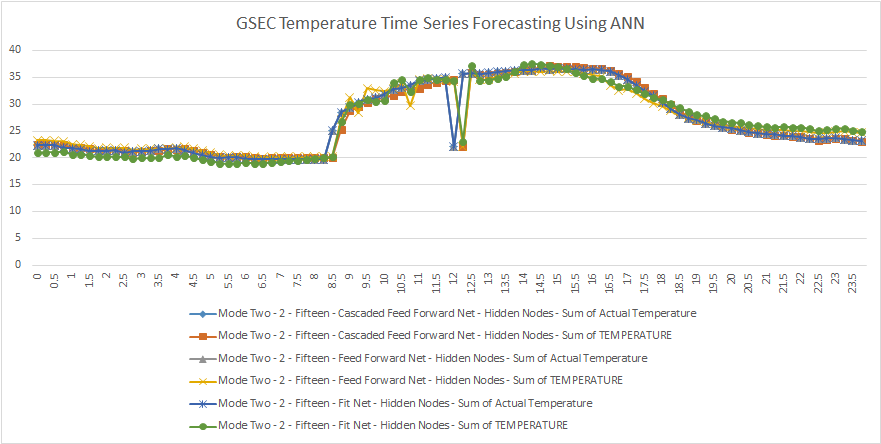
\includegraphics[scale=0.5]{ANNmTwo15t}
\caption{Comparison Of Different ANN Architectures (FN,FF,CFF) For Forecasting Of Intra-Hour Temperature In Mode 2 With Network [15]}
\label{ANNResImg30} %% to refer use, \ref{}
\end{figure}

\begin{figure}[H]
\centering
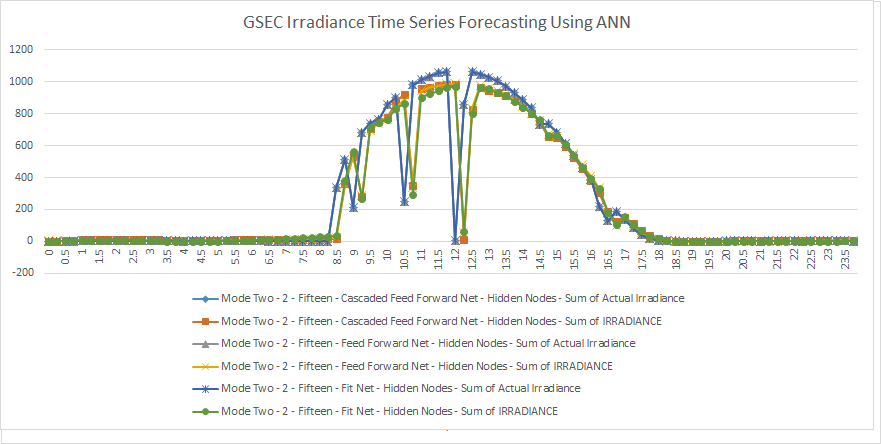
\includegraphics[scale=0.5]{ANNmTwo15i}
\caption{Comparison Of Different ANN Architectures (FN,FF,CFF) For Forecasting Of Intra-Hour Irradiance In Mode 2 With Network [15]}
\label{ANNResImg31} %% to refer use, \ref{}
\end{figure}

\begin{figure}[H]
\centering
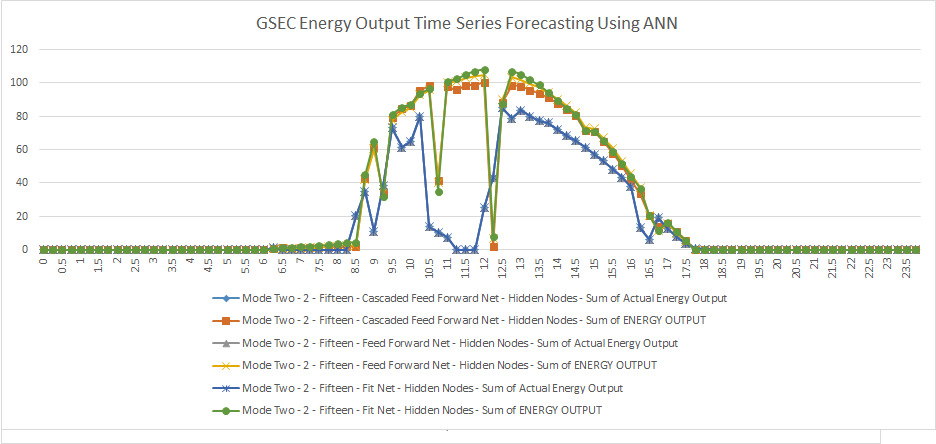
\includegraphics[scale=0.5]{ANNmTwo15e}
\caption{Comparison Of Different ANN Architectures (FN,FF,CFF) For Forecasting Of Intra-Hour Energy In Mode 2 With Network [15]}
\label{ANNResImg32} %% to refer use, \ref{}
\end{figure}


\subsubsection{ANN Architecture - Hidden Nodes [10-10]}
\
\
\
\

\begin{figure}[H]
\centering
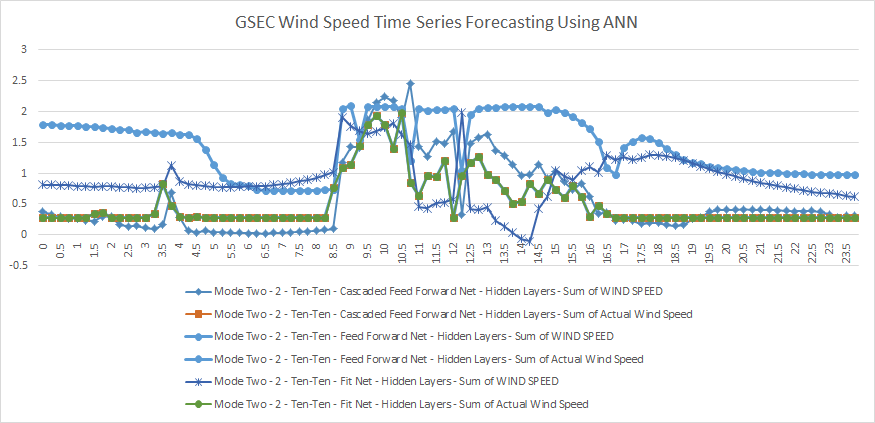
\includegraphics[scale=0.5]{ANNmTwo10-10w}
\caption{Comparison Of Different ANN Architectures (FN,FF,CFF) For Forecasting Of Intra-Hour Wind Speed In Mode 2 With Network [10-10]}
\label{ANNResImg33} %% to refer use, \ref{}
\end{figure}

\begin{figure}[H]
\centering
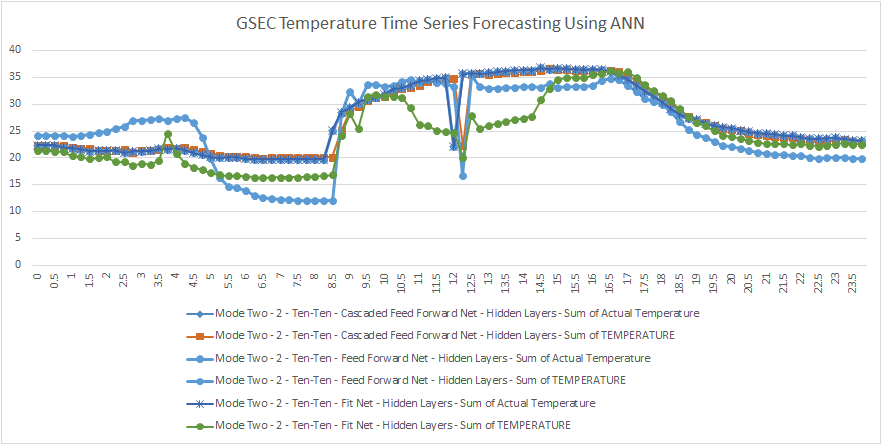
\includegraphics[scale=0.5]{ANNmTwo10-10t}
\caption{Comparison Of Different ANN Architectures (FN,FF,CFF) For Forecasting Of Intra-Hour Temperature In Mode 2 With Network [10-10]}
\label{ANNResImg34} %% to refer use, \ref{}
\end{figure}

\begin{figure}[H]
\centering
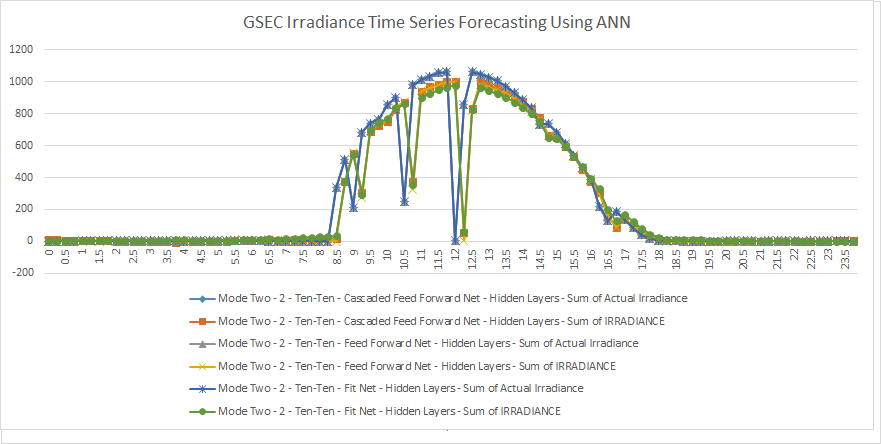
\includegraphics[scale=0.5]{ANNmTwo10-10i}
\caption{Comparison Of Different ANN Architectures (FN,FF,CFF) For Forecasting Of Intra-Hour Irradiance In Mode 2 With Network [10-10]}
\label{ANNResImg35} %% to refer use, \ref{}
\end{figure}

\begin{figure}[H]
\centering
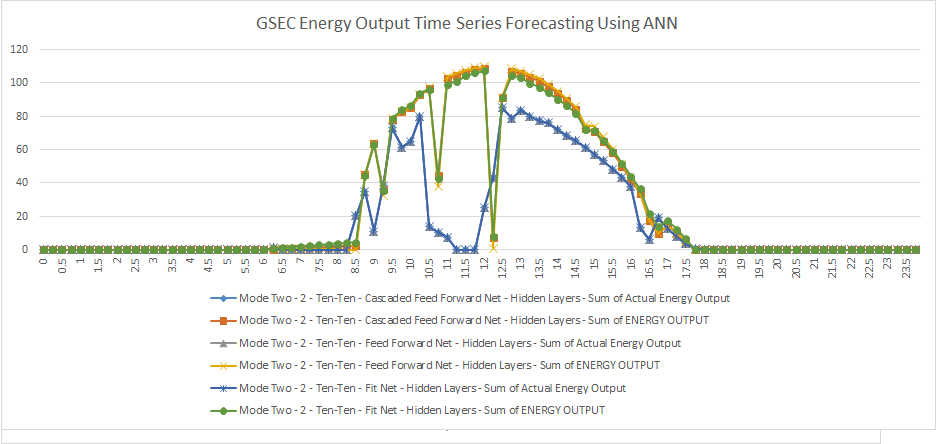
\includegraphics[scale=0.5]{ANNmTwo10-10e}
\caption{Comparison Of Different ANN Architectures (FN,FF,CFF) For Forecasting Of Intra-Hour Energy In Mode 2 With Network [10-10]}
\label{ANNResImg36} %% to refer use, \ref{}
\end{figure}

\subsubsection{ANN Architecture - Hidden Nodes [10-10-10]}
\
\
\
\

\begin{figure}[H]
\centering
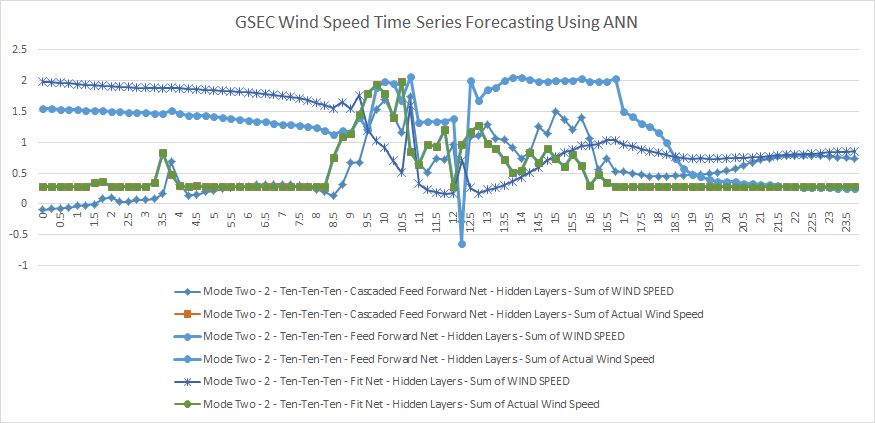
\includegraphics[scale=0.5]{ANNmTwo10-10-10w}
\caption{Comparison Of Different ANN Architectures (FN,FF,CFF) For Forecasting Of Intra-Hour Wind Speed In Mode 2 With Network [10-10-10]}
\label{ANNResImg37} %% to refer use, \ref{}
\end{figure}

\begin{figure}[H]
\centering
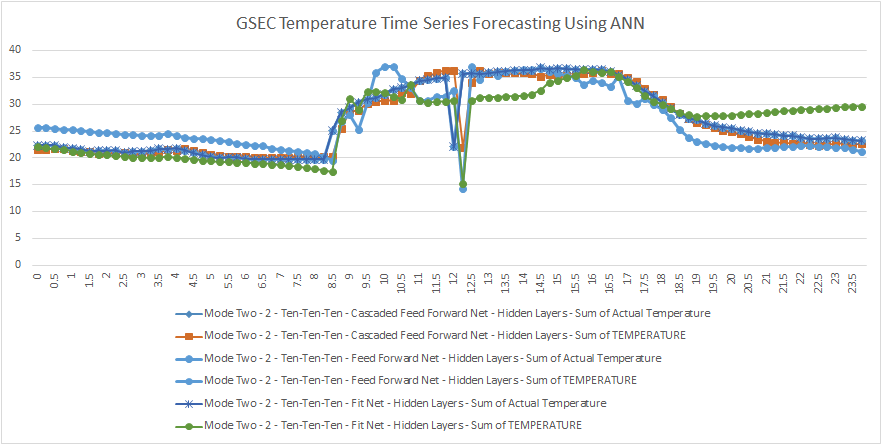
\includegraphics[scale=0.5]{ANNmTwo10-10-10t}
\caption{Comparison Of Different ANN Architectures (FN,FF,CFF) For Forecasting Of Intra-Hour Temperature In Mode 2 With Network [10-10-10]}
\label{ANNResImg38} %% to refer use, \ref{}
\end{figure}

\begin{figure}[H]
\centering
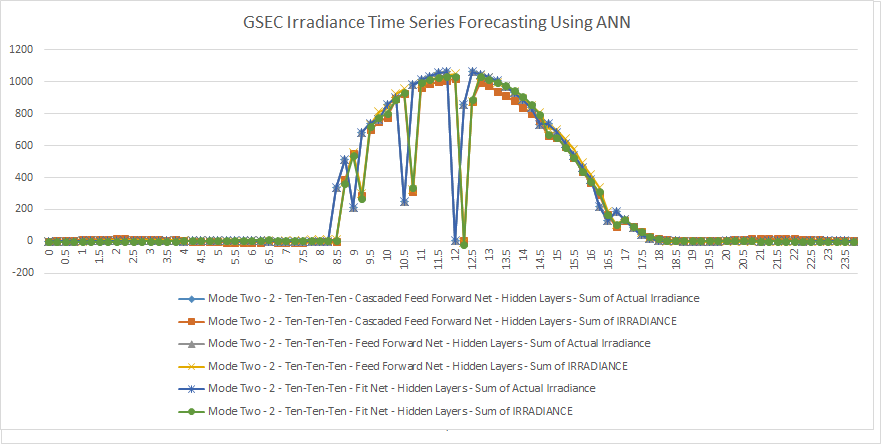
\includegraphics[scale=0.5]{ANNmTwo10-10-10i}
\caption{Comparison Of Different ANN Architectures (FN,FF,CFF) For Forecasting Of Intra-Hour Irradiance In Mode 2 With Network [10-10-10]}
\label{ANNResImg39} %% to refer use, \ref{}
\end{figure}

\begin{figure}[H]
\centering
\includegraphics[scale=0.5]{ANNmTwo10-10-10e}
\caption{Comparison Of Different ANN Architectures (FN,FF,CFF) For Forecasting Of Intra-Hour Energy In Mode 2 With Network [10-10-10]}
\label{ANNResImg40} %% to refer use, \ref{}
\end{figure}



\subsection{Input Type - Mode3}
\
\
\
\
In Mode2 the Input training matrix consists of the [Day, Month, Year,Time] columns with the Target Training Matrix consisting of the corresponding [Wind Speed, Temperature, Irradiance, Previous Wind Speed, Previous Temperature, Previous Irradiance, Rate of Change of Previous Wind Speed, Rate of Change of Previous Temperature, Rate of Change of Previous Irradiance] columns. The results are given in the following sections which are divided based on the hidden network configurations and each graph consists of the comparison of the actual variable with he forecasted variable from the three different ANN architectures. 

\subsubsection{ANN Architecture - Hidden Nodes [5]}
\
\
\
\

\begin{figure}[H]
\centering
\includegraphics[scale=0.5]{ANNmThree5w}
\caption{Comparison Of Different ANN Architectures (FN,FF,CFF) For Forecasting Of Intra-Hour Wind Speed In Mode 3 With Network [5]}
\label{ANNResImg41} %% to refer use, \ref{}
\end{figure}

\begin{figure}[H]
\centering
\includegraphics[scale=0.5]{ANNmThree5t}
\caption{Comparison Of Different ANN Architectures (FN,FF,CFF) For Forecasting Of Intra-Hour Temperature In Mode 3 With Network [5]}
\label{ANNResImg32} %% to refer use, \ref{}
\end{figure}

\begin{figure}[H]
\centering
\includegraphics[scale=0.5]{ANNmThree5i}
\caption{Comparison Of Different ANN Architectures (FN,FF,CFF) For Forecasting Of Intra-Hour Irradiance In Mode 3 With Network [5]}
\label{ANNResImg33} %% to refer use, \ref{}
\end{figure}

\begin{figure}[H]
\centering
\includegraphics[scale=0.5]{ANNmThree5e}
\caption{Comparison Of Different ANN Architectures (FN,FF,CFF) For Forecasting Of Intra-Hour Energy In Mode 3 With Network [5]}
\label{ANNResImg44} %% to refer use, \ref{}
\end{figure}

\newpage

\subsubsection{ANN Architecture - Hidden Nodes [10]}
\
\
\
\

\begin{figure}[H]
\centering
\includegraphics[scale=0.5]{ANNmThree10w}
\caption{Comparison Of Different ANN Architectures (FN,FF,CFF) For Forecasting Of Intra-Hour Wind Speed In Mode 3 With Network [10]}
\label{ANNResImg45} %% to refer use, \ref{}
\end{figure}

\begin{figure}[H]
\centering
\includegraphics[scale=0.5]{ANNmThree10t}
\caption{Comparison Of Different ANN Architectures (FN,FF,CFF) For Forecasting Of Intra-Hour Temperature In Mode 3 With Network [10]}
\label{ANNResImg46} %% to refer use, \ref{}
\end{figure}

\begin{figure}[H]
\centering
\includegraphics[scale=0.5]{ANNmThree10i}
\caption{Comparison Of Different ANN Architectures (FN,FF,CFF) For Forecasting Of Intra-Hour Irradiance In Mode 3 With Network [10]}
\label{ANNResImg47} %% to refer use, \ref{}
\end{figure}

\begin{figure}[H]
\centering
\includegraphics[scale=0.5]{ANNmThree10e}
\caption{Comparison Of Different ANN Architectures (FN,FF,CFF) For Forecasting Of Intra-Hour Energy In Mode 3 With Network [10]}
\label{ANNResImg48} %% to refer use, \ref{}
\end{figure}

\subsubsection{ANN Architecture - Hidden Nodes [15]}
\
\
\
\

\begin{figure}[H]
\centering
\includegraphics[scale=0.5]{ANNmThree15w}
\caption{Comparison Of Different ANN Architectures (FN,FF,CFF) For Forecasting Of Intra-Hour Wind Speed In Mode 3 With Network [15]}
\label{ANNResImg49} %% to refer use, \ref{}
\end{figure}

\begin{figure}[H]
\centering
\includegraphics[scale=0.5]{ANNmThree15t}
\caption{Comparison Of Different ANN Architectures (FN,FF,CFF) For Forecasting Of Intra-Hour Temperature In Mode 3 With Network [15]}
\label{ANNResImg50} %% to refer use, \ref{}
\end{figure}

\begin{figure}[H]
\centering
\includegraphics[scale=0.5]{ANNmThree15i}
\caption{Comparison Of Different ANN Architectures (FN,FF,CFF) For Forecasting Of Intra-Hour Irradiance In Mode 3 With Network [15]}
\label{ANNResImg51} %% to refer use, \ref{}
\end{figure}

\begin{figure}[H]
\centering
\includegraphics[scale=0.5]{ANNmThree15e}
\caption{Comparison Of Different ANN Architectures (FN,FF,CFF) For Forecasting Of Intra-Hour Energy In Mode 3 With Network [15]}
\label{ANNResImg52} %% to refer use, \ref{}
\end{figure}


\subsubsection{ANN Architecture - Hidden Nodes [10-10]}
\
\
\
\

\begin{figure}[H]
\centering
\includegraphics[scale=0.5]{ANNmThree10-10w}
\caption{Comparison Of Different ANN Architectures (FN,FF,CFF) For Forecasting Of Intra-Hour Wind Speed In Mode 3 With Network [10-10]}
\label{ANNResImg53} %% to refer use, \ref{}
\end{figure}

\begin{figure}[H]
\centering
\includegraphics[scale=0.5]{ANNmThree10-10t}
\caption{Comparison Of Different ANN Architectures (FN,FF,CFF) For Forecasting Of Intra-Hour Temperature In Mode 3 With Network [10-10]}
\label{ANNResImg54} %% to refer use, \ref{}
\end{figure}

\begin{figure}[H]
\centering
\includegraphics[scale=0.5]{ANNmThree10-10i}
\caption{Comparison Of Different ANN Architectures (FN,FF,CFF) For Forecasting Of Intra-Hour Irradiance In Mode 3 With Network [10-10]}
\label{ANNResImg55} %% to refer use, \ref{}
\end{figure}

\begin{figure}[H]
\centering
\includegraphics[scale=0.5]{ANNmThree10-10e}
\caption{Comparison Of Different ANN Architectures (FN,FF,CFF) For Forecasting Of Intra-Hour Energy In Mode 3 With Network [10-10]}
\label{ANNResImg56} %% to refer use, \ref{}
\end{figure}

\subsubsection{ANN Architecture - Hidden Nodes [10-10-10]}
\
\
\
\

\begin{figure}[H]
\centering
\includegraphics[scale=0.5]{ANNmThree10-10-10w}
\caption{Comparison Of Different ANN Architectures (FN,FF,CFF) For Forecasting Of Intra-Hour Wind Speed In Mode 3 With Network [10-10-10]}
\label{ANNResImg57} %% to refer use, \ref{}
\end{figure}

\begin{figure}[H]
\centering
\includegraphics[scale=0.5]{ANNmThree10-10-10t}
\caption{Comparison Of Different ANN Architectures (FN,FF,CFF) For Forecasting Of Intra-Hour Temperature In Mode 3 With Network [10-10-10]}
\label{ANNResImg58} %% to refer use, \ref{}
\end{figure}

\begin{figure}[H]
\centering
\includegraphics[scale=0.5]{ANNmThree10-10-10i}
\caption{Comparison Of Different ANN Architectures (FN,FF,CFF) For Forecasting Of Intra-Hour Irradiance In Mode 3 With Network [10-10-10]}
\label{ANNResImg59} %% to refer use, \ref{}
\end{figure}

\begin{figure}[H]
\centering
\includegraphics[scale=0.5]{ANNmThree10-10-10e}
\caption{Comparison Of Different ANN Architectures (FN,FF,CFF) For Forecasting Of Intra-Hour Energy In Mode 3 With Network [10-10-10]}
\label{ANNResImg60} %% to refer use, \ref{}
\end{figure}

\subsubsection{Conclusion from Graphs}
\
\
\
\
It is observed from the above graphs that as the input training set holds more and more data about the previous states of the weather variables to be forecasted the model learning for one-step ahead generation forecasting becomes better and better even with less complex network architectures. It is seen that the learning and model generalization are better with increasing complexity of the hidden network architecture as deep learning takes place. Moreover, the learning is least affected by the use of the different ANN architectures as FN, FF and CFF all fall in the same family of Multi-Layer Perceptron Models. The use of Radial Bias Functions has to be explored to have a more clear understanding of which ANN architecture is better suite for the job.


